\documentclass[]{scrartcl}

\usepackage[sort, square]{natbib}
\usepackage{hyperref}
\usepackage{amsmath}
\usepackage{graphicx}
\usepackage{amsmath}
\usepackage{amssymb}
\usepackage{amsfonts}
% sichert die richtige Darstellung der deutschen Sprache
\usepackage[ngerman]{babel}
\usepackage[utf8]{inputenc}
\usepackage[T1]{fontenc}
% % % % % % % %
\usepackage{multirow}
\usepackage{geometry}
\usepackage{setspace}
\usepackage{siunitx}
\usepackage{textcomp}
\usepackage{colortbl}
\usepackage{extarrows}

\newcommand\abb[1]{\textbf{\underline{#1}}}
% Startet neue Seite pro \section{} Befehl
\usepackage{titlesec}
\newcommand{\sectionbreak}{\clearpage}
% % % % % % % %

\usepackage{pgf}
\usepackage{color}
\definecolor{mygray}{rgb}{0.5,0.5,0.5}
\definecolor{LimeGreen}{HTML}{9EFD38}
\usepackage{cancel}
\usepackage{url}
\usepackage{epstopdf}
\sisetup{ output-decimal-marker = {,}} % Decimalzahlen sind durch Komma getrennt

% Ein Caption für ein Listing wird definiert
\usepackage{caption}
\usepackage{listings}

\DeclareCaptionFont{white}{ \color{white} }
\DeclareCaptionFormat{listing}{
	\colorbox[cmyk]{0.43, 0.35, 0.35,0.01 }{
		\parbox{\textwidth}{\hspace{15pt}#1#2#3}
	}
}
\captionsetup[lstlisting]{ format=listing, labelfont=white, textfont=white, singlelinecheck=false, margin=0pt, font={bf,footnotesize} }
% % % % % % % % % % % % % % % % % % % % % % % % % % % % % % % % % % % %


\geometry{outer=30mm,
inner=30mm,
top=20mm,
bottom=30mm}

\newcommand\grad{^{\circ}}
% 
%
% Unterstreichen und Umrahmen der Formeln in align-Umgebung
\newcommand\ul[2][]{%Befehl zum Unterstreichen von #2 mit eventueller Größenabstimmung mit #1 
 \underline{#2\vphantom{#1}}}%wenn #1 angegeben, wird Tiefe der Linie angepaßt 

\newcommand\ulalign[2]{\ul[#2]{#1}&\ul[#1]{\;=#2}}%einfaches Unterstreichen einer align-Gl. mit &= 
\newcommand\dulalign[2]{\underline{\ul[#2]{#1}}&\underline{\ul[#1]{\;=#2}}}%doppeltes Unterstreichen einer align-Gl. mit &= 


\usepackage{tikz} 
\usetikzlibrary{fit} 

\newcommand\raalign[2]{%Umrahmen einer align-Gl. mit &= 
   \tikz[overlay,every node/.style={inner sep=0pt,outer sep=0pt}]% 
      \node[anchor=base west](g){\phantom{$\displaystyle #1\null=\null#2$}}% 
         node[draw=gray!70!black,fill=gray!20,fit=(g),inner sep=5pt]{};% 
   #1&=#2} 
  
% 
%
% 


\usepackage{listings} % Quellcode im Text
\lstset{language=JAVA, % Programmiersprache
		tabsize=1, 	  % Länge des Tab Zeichens
        basicstyle=\ttfamily\color{mygray}\small, % style des Codes
        keywordstyle=\ttfamily\color{blue},
        identifierstyle=\color{mygray},
        commentstyle=\color{red},
        stringstyle=\ttfamily\color{black},
        showstringspaces=false,
        numbers=left, 
        numberstyle=\tiny, 
        stepnumber=1, 
        numbersep=5pt,
        breaklines=true,
        literate=%   
            {Ö}{{\"O}}1
            {Ä}{{\"A}}1
            {Ü}{{\"U}}1
            {ß}{{\ss}}1
            {ü}{{\"u}}1
            {ä}{{\"a}}1
            {ö}{{\"o}}1
            {~}{{\textasciitilde}}1}

\newcommand{\HRule}{\rule{\linewidth}{0.5mm}}


\usepackage[tocflat]{tocstyle}   
\usetocstyle{allwithdot}

\begin{document}
	
\begin{titlepage}
	
	\begin{center}
		
		\textsc{\LARGE Dokumentation}\\[2cm]
		\textsc{\large im Studiengang Informationstechnik}\\
		der\\
		\textsc{\large Dualen Hochschule Baden-Württemberg}\\
		\textsc{\large Standort Stuttgart}\\
		\textsc{\large Software-Engineering}\\[3.2cm]
		
		%\includegraphics[width=\textwidth]{./Logo.eps}\\[1cm]

		\HRule \\[0.4cm]
		{\huge \bfseries Webbasiertes Bewertungssystem PASS}\\[0.4cm]
		\HRule \\[0.1cm]
		\author{\vhListAllAuthors}
		\large von:\\ \textsc{\sLong}\\[0.2cm]
		(Version \vhCurrentVersion\hspace{0.1cm} vom \vhCurrentDate)
		\vspace{10.0cm}
			
	\end{center}

\end{titlepage}
	\tableofcontents
	\newpage

	\section{Zielbestimmung}
		\subsection{Musskriterien}
			
			\begin{itemize}
			\item[-]	Verschiedene Benutzergruppen 
			\item[-]	Benutzer anlegen
			\item[-]	Rechtehierarchien
			\item[-]	Studenten können ihre Noten in dem System einsehen.
			\item[-]	Notenkonvertierungsprofile erstellen und verwalten
			\item[-]	Dozenten weisen einer Veranstaltung Bewertungsschema zu
			\item[-]	Ein Template kann zu einer Veranstaltung erstellt werden.
			\item[-]	Veranstaltungen des Typs (Gruppenarbeit, Einzelarbeit) können erstellt werden.
			\item[-]	Die Festlegung eines Grundscore (Gruppe, einzeln) lässt sich in zwei skalierbare \newline Bereiche beliebig teilen ($H_2$)
			\item[-]	Score Refining Faktoren können in einem Template frei eingestellt werden (Items) ($R_2S$)
			\item[-]	Skalierbarkeit des Bewertungssystems von Bewertung der Gruppe zu Einzelperson und umgekehrt.
			\item[-]	Zuweisung von beliebig gruppierten Studenten zu einer \item[-]	Veranstaltung durch Dozent oder Prüfer.				
			\end{itemize}

			
		\subsection{Wunschkriterien}
		\begin{itemize}
		\item[-]	Alle Zwischenbewertungen die zur Note führen werden dem Studenten angezeigt.
		\item[-]	Profilverwaltung um standardisierte Bewertungen erzeugen zu können.
		\end{itemize}
		
		\subsection{Abgrenzungskriterien}
		\begin{itemize}
		\item[-]	Bewertungssystem bewertet nur die Veranstaltungen die einer Art bestanden/nicht bestanden Logik unterliegen. Anschließend erfolgt eine konfigurierbare Punkte-Notenkonvertierung.
		\item[-]	Jede erstellte Veranstaltung beinhaltet genau ein Bewertungsschema und führt somit zu einer Note. Die Kombinierbarkeit von verschiedenen Einzelnoten ist nicht möglich.
		\end{itemize}
		
	\section{Produkteinsatz}
	
		
		\subsection{Anwendungsbereiche}
		\begin{itemize}
		\item[-]	Planung einer Veranstaltung mit anstehenden Prüfungsleistungen für Lehrveranstaltungsplaner
		\item[-]	Errechnung einer Note durch den Prüfer anhand festgelegter Kriterien.
		\item[-]	Einsicht der Noten durch Studenten, sowie die Leistungsübersicht für die Dozenten und Prüfer.
		\end{itemize}
		
		
		\subsection{Zielgruppen}
		\begin{itemize}
		\item[-]	Lehrveranstaltungsplaner
		\item[-]	Prüfer
		\item[-]	Studenten
		\end{itemize}

		\subsection{Betriebsbedingungen}
		\begin{itemize}
		\item[-]	Das System soll nur einmal angelegt werden und autark funktionieren.
		\item[-]	Klar definierte Benutzergruppen und Rechte
		\item[-]	Datenbankschnittstelle für Benutzerverwaltung
		\item[-]	Datenbank-Umgebung für die Speicherung der Daten
		\item[-]	Archivierung der Daten (Datensicherheit wegen Einsehbarkeit der Daten)
		\item[-]	Zugriff von außen sowohl als Lesen, als auch als Edit möglich. 
		\end{itemize}

		
		
		
		
	\section{Produktübersicht}
	
	Das Produkt wird durch folgende Use Cases definiert. Die Anforderung an die Funktionalität ensteht aus der Auswertung der Akteur/Produkt- und Akteur/Akteur-Beziehungen.
	
	\subsection{Use Case Analyse}
	
	\begin{table}[ht!]
	\begin{tabular}{ll}
	 \textbf{Use Case ID} & 1 \\
 	 \textbf{Elementarer Geschäftsprozess} & /F10/ Veranstaltung planen \\ 
	 \textbf{Ziel des Use Cases} & Darstellung des  Prozesses einer    \\
	 & Veranstaltungsplanung\\ 
	 \textbf{Umgebende Systemgrenze}& Veranstaltungskonfigurator \\ 
	 \textbf{Vorbedingung} & Dozent ist angemeldet \\ 
	 \textbf{Nachbedingung Erfolg} & Veranstaltung ist angelegt \\ 
	 & Template ist erstellt\\
	 \textbf{Beteiligte Nutzer:} & Dozent \\ 
     \textbf{Auslösendes Ereignis:} & Dozent möchte Veranstaltung planen \\ 
	 
	\end{tabular} 
	\label{tab:usecase_1}
	\end{table}
	
		\begin{table}[ht!]
		\begin{tabular}{ll}
		 \textbf{Use Case ID} & 2 \\
	 	 \textbf{Elementarer Geschäftsprozess} & /F20/ Template erstellen \\ 
		 \textbf{Ziel des Use Cases} & Templates für die Veranstaltungen können \\& angelegt werden   \\
		 \textbf{Umgebende Systemgrenze}& Veranstaltungskonfigurator \\ 
		 \textbf{Vorbedingung} & Dozent ist angemeldet \\ 
		 \textbf{Nachbedingung Erfolg} & Template ist erstellt \\ 
		 \textbf{Beteiligte Nutzer:} & Dozent \\ 
	     \textbf{Auslösendes Ereignis:} & Dozent möchte Template erstellen \\ 
		 
		\end{tabular} 
		\label{tab:usecase_2}
		\end{table}
	
	
			\begin{table}[ht!]
			\begin{tabular}{ll}
			 \textbf{Use Case ID} & 3 \\
		 	 \textbf{Elementarer Geschäftsprozess} & /F20/ Bewerten \\ 
			 \textbf{Ziel des Use Cases} & Prüfer bewertet  \\
			 \textbf{Umgebende Systemgrenze} & Bewertung \\ 
			 \textbf{Vorbedingung} & Veranstaltung existiert \\
			  					   & Studenten/Gruppen existieren \\ 
			 \textbf{Nachbedingung Erfolg} & Teilbewertung liegt vor \\
			 							   & Bewertung ist abgeschlossen\\
			 							    
			 \textbf{Beteiligte Nutzer:} & Prüfer \\ 
		     \textbf{Auslösendes Ereignis:} & Prüfer will Gruppe/Student bewerten \\ 
			 
			\end{tabular} 
			\label{tab:usecase_3}
			\end{table}
			
			\begin{table}[ht!]
			\begin{tabular}{ll}
			 \textbf{Use Case ID} & 4 \\
		 	 \textbf{Elementarer Geschäftsprozess} & /F20/ Einsehen \\ 
			 \textbf{Ziel des Use Cases} & Studenten sehen ihre Noten ein  \\
			 \textbf{Umgebende Systemgrenze} & Bewertung \\ 
			 \textbf{Vorbedingung} & Bewertung liegt bereits vor \\
			 \textbf{Nachbedingung Erfolg} & Student sieht die Note\\
			 			    
			 \textbf{Beteiligte Nutzer:} & Student \\ 
		     \textbf{Auslösendes Ereignis:} & Student will seine Note sehen\\ 
			 
			\end{tabular} 
			\label{tab:usecase_4}
			\end{table}
			
			\begin{table}[ht!]
			\begin{tabular}{ll}
			 \textbf{Use Case ID} & 5 \\
		 	 \textbf{Elementarer Geschäftsprozess} & /F20/ Teilnehmer anlegen \\ 
			 \textbf{Ziel des Use Cases} & Prüfer oder Dozent konfigurieren \\& die Teilnehmer einer Veranstaltung  \\
			 \textbf{Umgebende Systemgrenze} & Planung Prüfung \\ 
			 \textbf{Vorbedingung} & Veranstaltung ist konfiguriert \\
			 \textbf{Nachbedingung Erfolg} & Veranstaltung ist freigegeben\\
			 			    
			 \textbf{Beteiligte Nutzer:} & Prüfer,Dozent \\ 
		     \textbf{Auslösendes Ereignis:} & Studenten sollen einer Veranstaltung hinzugefügt werden\\ 
			 
			\end{tabular} 
			\label{tab:usecase_5}
			\end{table}

						
		\clearpage
		\subsection{Use Cases in grafischer Darstellung}
		
	\begin{figure}[th!]
	\centering
	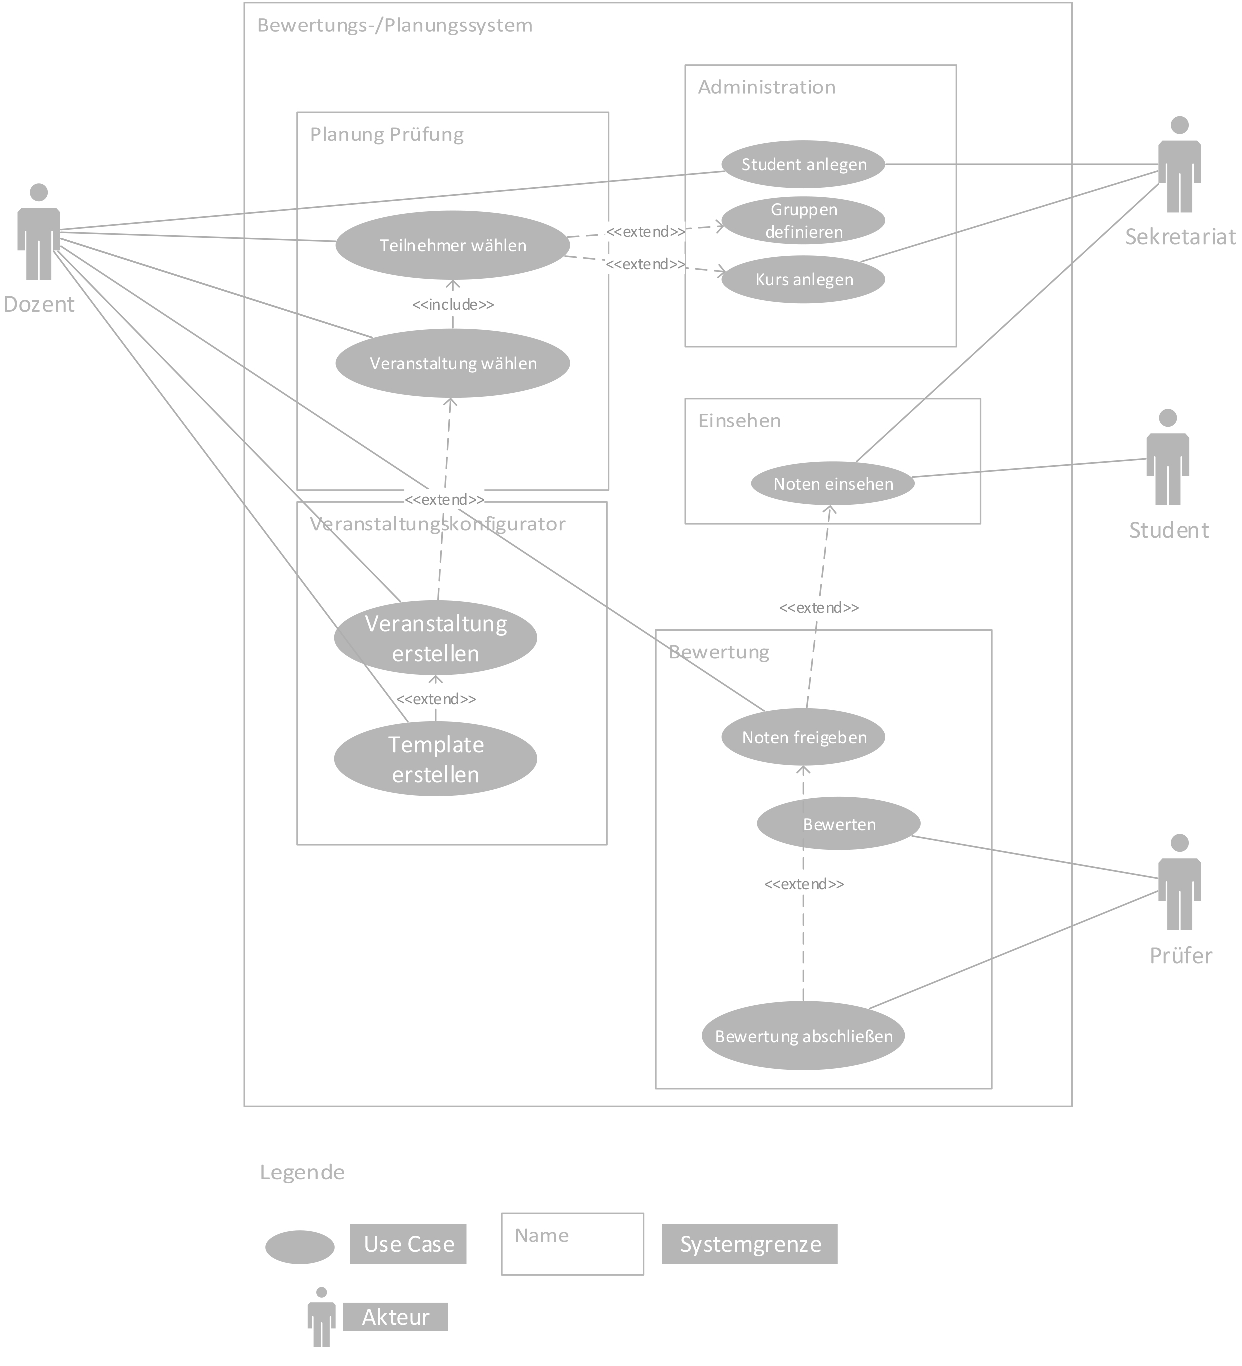
\includegraphics[width=\textwidth]{./img/use_case}
	\caption{Darstellung des Gesamtsystems anhand der ausgearbeiteten Use-Cases}
	\label{fig:use_case}
	\end{figure}
	

	
	\begin{figure}[th!]
	\centering
	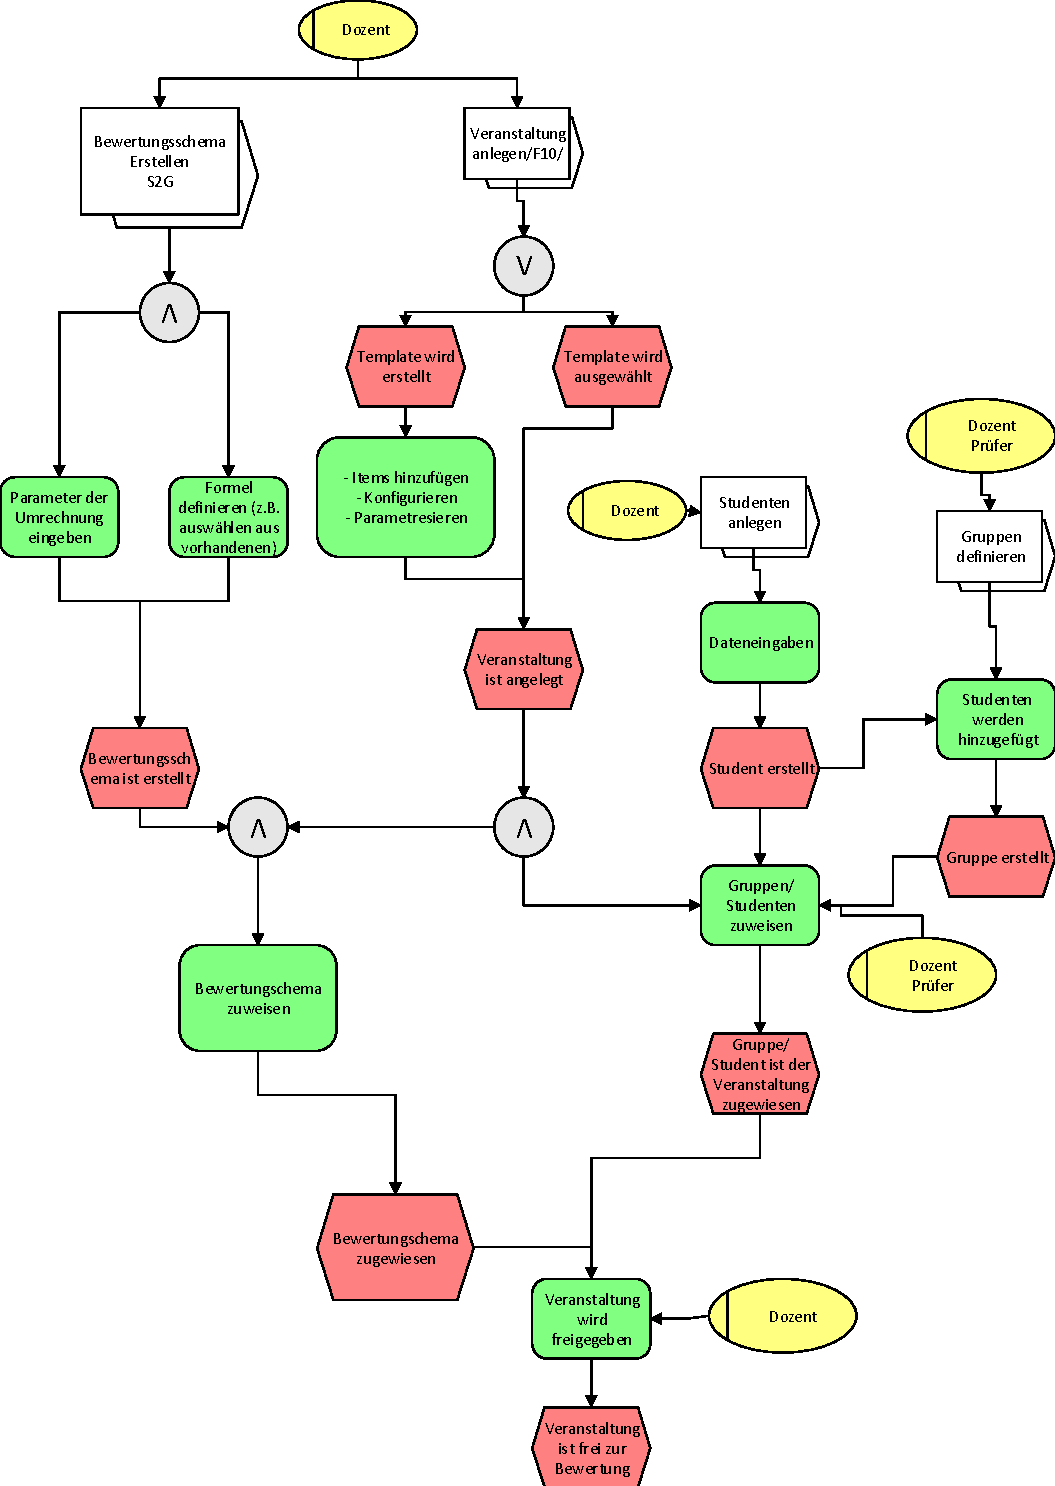
\includegraphics[width=\textwidth]{./img/ablauf_1}
	\caption{Prozessdiagramm für Geschäftsprozess Veranstaltungserstellung}
	\label{fig:process1}
	\end{figure}
		
	\begin{figure}[th!]
	\centering
	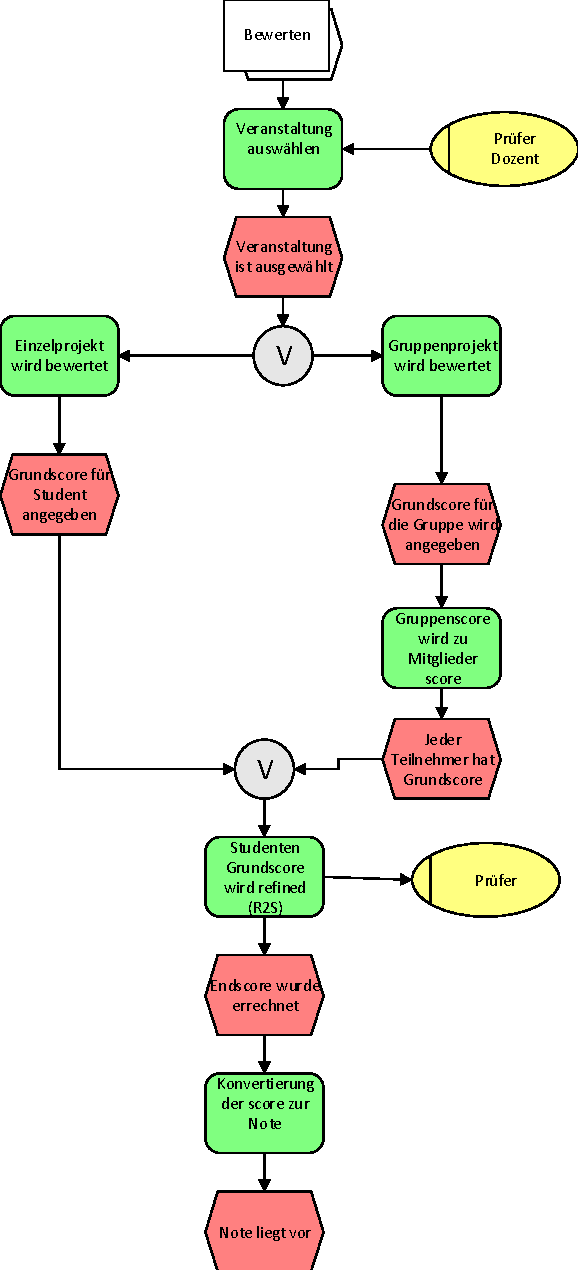
\includegraphics[width=0.6\textwidth]{./img/ablauf_2}
	\caption{Ablaufdiagramm für den Geschäftsprozess Bewertung}
	\label{fig:process2}
	\end{figure}

	\section{Produktfunktionen}
	Im folgenden sind die Produktfunktionen aus den Ablaufdiagrammen dokumentiert. Diese werden im Laufe der Entwicklung angepasst und in ihrem Umfang erweitert.
	
	\begin{table}[ht]
	\begin{tabular}{ll}
		\multicolumn{2}{l}{/\textbf{\textit{F10}}/}\\\hline
		 \textbf{Geschäftsprozess} & Veranstaltung planen \\ 
		 \textbf{Kategorie} & primär \\ 
		 \textbf{Vorbedingung} & Dozent ist angemeldet\\
		 & ein Template liegt vor \\ 
		  	& Bewertungsschema liegt vor\\
		 	& Prüfer liegen vor\\
		 \textbf{Nachbedingung Erfolg} & Eine Veranstaltung ist angelegt  \\ 
		 & Prüfer erfährt welchen Kurs (bzw.  Student/en) er zu prüfen hat.\\
		 \textbf{Nachbedingung Fehlschlag} &  \\ 
		 \textbf{Akteure} & Dozent \\ 
		 \textbf{Auslösendes Ereignis} & Dozent legt eine Veranstaltung an  \\ 
		 \textbf{Beschreibung} &  1. Dozent konfiguriert das Template\\ 
		 & 2. Dozent befüllt(prüft) die Parameter des Bewertungsschemas\\
		 & 3. Dozent kann Prüfer einer Veranstaltung zuteilen zuteilen \\
		 & 4. Dozent kann Studenten/Gruppen der  Veranstaltung zuweisen\\
		  \textbf{Erweiterung} &  \\ 
		 \textbf{Alternativen} & 1. Neues Template anlegen \\
		 & 2. Neue Studenten anlegen\\
		 & 3. Neue Prüfer Anlegen \\
		 & 4. Neues Bewertungsschema anlegen
		 \end{tabular} 
	\label{tab:F10}
	\end{table}
	
		\begin{table}[ht]
		\begin{tabular}{ll}
			\multicolumn{2}{l}{/\textbf{\textit{F20}}/}\\\hline
			 \textbf{Geschäftsprozess} & Template erstellen \\ 
			 \textbf{Kategorie} & primär \\ 
			 \textbf{Vorbedingung} & Dozent ist angemeldet\\
			 & ein Bewertungsschema liegt vor \\ 

			 \textbf{Nachbedingung Erfolg} & Template ist
			  zur Veranstaltungsplanung freigegeben  \\ 
			 \textbf{Nachbedingung Fehlschlag} &  \\ 
			 \textbf{Akteure} & Dozent \\ 
			 \textbf{Auslösendes Ereignis} & Dozent legt ein Template an \\
			 & Bei Veranstaltungserstellung wurde kein Template gefunden\\
			 & Bei Veranstaltungserstellung wird ein neues Template erstellt\\
			 \textbf{Beschreibung} & 1. Die Art der Prüfung wird spezifiziert \\
			 & 2. Items hinzufügen\\
			 & 3. Bewertungsschema hinzufügen\\
			  \textbf{Erweiterung} & 1. Templates refactoring \\ 
			 \textbf{Alternativen} & 1. Neues Bewertungsschema erstellen anlegen \\  			
			 \end{tabular} 
		\label{tab:F20}
		\end{table}
	
		\begin{table}[ht]
		\begin{tabular}{ll}
			\multicolumn{2}{l}{/\textbf{\textit{F30}}/}\\\hline
			 \textbf{Geschäftsprozess} & Bewertungsschema festlegen \\ 
			 \textbf{Kategorie} & primär \\ 
			 \textbf{Vorbedingung} & 1. Dozent ist angemeldet  \\ 
			 \textbf{Nachbedingung Erfolg} & Ein Bewertungsschema steht zur Verfügung\\ 
			 & Prüfer erfährt welchen Kurs (bzw.  Student/en) er zu prüfen hat.\\
			 \textbf{Akteure} & Dozent \\ 
			 \textbf{Auslösendes Ereignis} & Dozent legt ein Bewertungsschema an  \\ 
			 \textbf{Beschreibung} &  1. Umrechnungsformel festlegen\\
			 & 2. Parameter anpassen
			 \end{tabular} 
		\label{tab:F30}
		\end{table}
	
	
			\begin{table}[ht]
			\begin{tabular}{ll}
				\multicolumn{2}{l}{/\textbf{\textit{F40}}/}\\\hline
				 \textbf{Geschäftsprozess} & Bewerten \\ 
				 \textbf{Kategorie} & primär \\ 
				 \textbf{Vorbedingung} & 1. Dozent/Prüfer ist angemeldet  \\ 
				 & 2. Veranstaltung ist angelegt\\
				 & 3. Gruppen/Student ist einer Veranstaltung zugewiesen\\
				 & 4. Prüfer ist einer Veranstaltung zugewiesen\\
				 \textbf{Nachbedingung Erfolg} & Ein Student/Gruppe wurde bewertet\\
				 & Teilbewertung/vollständige Bewertung ist abgeschlossen\\ 
				 \textbf{Akteure} & Dozent \\ 
				 & Prüfer\\
				 \textbf{Auslösendes Ereignis} & Prüfer will bewerten \\ 
				 \textbf{Beschreibung} &  1. Prüfer wählt Veranstaltung aus\\
				 & Prüfer wählt Student/Gruppe zur Bewertung aus\\
				 & Bewertungen/Teilbewertungen eintragen\\
				 & Bewertung abschließen\\
			
				 \end{tabular} 
			\label{tab:F40}
			\end{table}
			
\begin{table}[ht]
	\begin{tabular}{ll}
		\multicolumn{2}{l}{/\textbf{\textit{F50}}/}\\\hline
		 \textbf{Geschäftsprozess} & Bewertung abschließen\\ 
		 \textbf{Kategorie} & primär \\ 
		 \textbf{Vorbedingung} & Bewertungen einer Veranstaltung in allen Items liegen vor\\
		 & Bewertungen für einen Student/Gruppe sind komplett\\
		 & Prüfer ist angemeldet \\ 
		 \textbf{Nachbedingung Erfolg} & Dozent erfährt, dass die Endnote der Veranstaltung vorliegt  \\ 
		 & Prüfer verliert das Recht zu editieren, nur noch sehen\\
		 & Nur Dozent ist berechtigt zu ändern\\
		 \textbf{Nachbedingung Fehlschlag} &  Die Bewertung steht weiter aus\\
		 & Bestätigung für den Abschluss trotz der \\
		 & unvollständigen Daten wird erfragt\\ 
		 \textbf{Akteure} & Dozent \\ 
		 & Prüfer\\
		 \textbf{Auslösendes Ereignis} & Prüfer schließt die Bewertung ab \\ 
		 \textbf{Alternativen} & 1. Bewertung vervollständigen \\
		 \end{tabular} 
	\label{tab:F50}
	\end{table}		
			
	\begin{table}[ht]
		\begin{tabular}{ll}
			\multicolumn{2}{l}{/\textbf{\textit{F60}}/}\\\hline
			 \textbf{Geschäftsprozess} & Kurs anlegen\\ 
			 \textbf{Kategorie} & primär \\ 
			 \textbf{Vorbedingung} & 1. Dozent ist angemeldet \phantom{aaaaaaaaaaaaaaaaaaaaaaaaaaaaaaa} \\
			  & Studenten liegen vor\\
			 \textbf{Nachbedingung Erfolg} & Kurs ist angelegt\\
			 \textbf{Nachbedingung Fehlschlag} & -\\
			 \textbf{Akteure} & Dozent \\ 
			 \textbf{Auslösendes Ereignis} & Dozent legt einen Kurs an\\ 
			 \textbf{Beschreibung} &  1. Kurs erstellen\\
			 & 2. Studenten hinzufügen\\
			 & 3. Kurs erstellen\\
			 \textbf{Alternativen} & 1. Studenten anlegen \\
			 \end{tabular} 
		\label{tab:F60}
		\end{table}
		
		
			\begin{table}[ht]
				\begin{tabular}{ll}
					\multicolumn{2}{l}{/\textbf{\textit{F70}}/}\\\hline
					 \textbf{Geschäftsprozess} & Studenten anlegen\\ 
					 \textbf{Kategorie} & primär \\ 
					 \textbf{Vorbedingung} & 1. Dozent ist angemeldet \phantom{aaaaaaaaaaaaaaaaaaaaaaaaaaaaaaa} \\
					 \textbf{Nachbedingung Erfolg} & Ein Student ist angelegt\\
					 & Student kann einem Kurs/Gruppe hinzugefügt werden\\
					 \textbf{Nachbedingung Fehlschlag} & -\\
					 \textbf{Akteure} & Dozent \\ 
					 \textbf{Auslösendes Ereignis} & Dozent legt Studenten an\\ 
					 \textbf{Beschreibung} &  1. Studentenregisterkarte erstellen\\
					 & 2. Daten befüllen\\
				 \end{tabular} 
				\label{tab:F70}
				\end{table}	
			
			\begin{table}[ht]
				\begin{tabular}{ll}
					\multicolumn{2}{l}{/\textbf{\textit{F80}}/}\\\hline
					 \textbf{Geschäftsprozess} & Bewertung einsehen\\ 
					 \textbf{Kategorie} & primär \\ 
					 \textbf{Vorbedingung} & 1. Student ist angemeldet \phantom{aaaaaaaaaaaaaaaaaaaaaaaaaaaaaaa} \\
					 &2. Bewertung liegt vor\\
					 \textbf{Nachbedingung Erfolg} & 1. Student sieht seine Noten\\
					  \textbf{Nachbedingung Fehlschlag} & Benachrichtigung\\
					 \textbf{Akteure} & Student \\ 
					 \textbf{Auslösendes Ereignis} & Student will seine Noten einsehen\\ 
					 \textbf{Beschreibung} &  1. Student meldet sich an\\
					 & 2. Student sieht seine Noten\\
				 \end{tabular} 
				\label{tab:F80}
				\end{table}	


	
	
	\section{Produktdaten}
	
		Die Größe der einzelnen Datenpunkte richtet sich variabel nach der letztendlichen Größe des Anwendungssystems. Die praktische Obergrenze wird durch die Hardware bzw. Datenbank festgelegt. 
	
	\begin{description}[\setlabelphantom{xxxxxx}]
	\item[/D10/] Benutzer \{Benutzer\_id, Benutzerart(Rechte) , Personendaten, Veranstaltungen\}\\ (Max. 100000) 
	\item[/D20/] Veranstaltung \{Veranstaltungs\_id, Bewertungsschema(S$_2$G), Bewertungstemplate, Prüfer, Stundenten, Score, Note, Status\_Bewertung\, Beschreibung\} \\ (Max. 100000)
	\item[/D30/] GUI-Daten (mehrere verschiedene Ansichten) \\
	Genauere Spezifikation erfolgt im zweiten Teil des Projekts im 4. Semester
	\item[/D40/] Datenarchiv {AlleDaten}
	
	\end{description}
	
	\section{Produktleistungen}
	
	\begin{description}[\setlabelphantom{xxxxxxx}]
	\item[/L10/] Die Antwortzeiten der Anwendung sollen so gering wie möglich gehalten werden.
	\item[/L20/] 	Die steigenden Benutzerzahlen die zur gleichen Zeit auf das System zugreifen, sollen jedoch keine signifikanten Einflüsse auf die Antwortzeiten des Systems haben.
	\item[/L30/]	Benutzerfreundliche UX soll implementiert werden.
	\item[/L40/]	Anbindung an bereits vorhandene Datenbanken soll in Zukunft möglich sein (wird im Prototypen zunächst nicht implementiert)
	\item[/L50/] 	Die Abfragen und die Einsicht der Daten von Außerhalb (WWW) ist entsprechend der Benutzerberechtigung möglich. (wird im Prototypen zu einem späteren Zeitpunkt realisiert)
	\item[/L60/] 	Datenbeständigkeit soll garantiert werden.
	\end{description}


	
	\section{Qualitätsanforderungen}
	\begin{table}[ht]
	\caption{Qualitätsmerkmale nach DIN ISO 9126 – siehe Anhang A in T3-4}
	\centering
		\begin{tabular}{|c|c|c|c|c|}
		\hline Produktqualität & sehr gut & gut & normal & nicht relevant \\ 
		\hline \multicolumn{5}{|c|}{Funktionalität}   \\ 
		\hline Angemessenheit &  &  & \checkmark &  \\ 
		\hline Richtigkeit &  & \checkmark  &  &  \\ 
		\hline Interoperabilität &  &\checkmark   &  &  \\ 
		\hline Ordnungsmäßigkeit &  &\checkmark   &  &  \\ 
		\hline Sicherheit &  &  & \checkmark  &  \\ 
		\hline \multicolumn{5}{|c|}{Zuverlässigkeit}   \\ 
		\hline Reife &  &   & \checkmark &  \\ 
		\hline Fehlertoleranz &  \checkmark &  &  &  \\ 
		\hline Wiederherstellbarkeit & \checkmark  &  &  &  \\ 
		\hline \multicolumn{5}{|c|}{Benutzbarkeit}  \\ 
		\hline Verständlichkeit &  &  & \checkmark  &  \\ 
		\hline Erlernbarkeit &  &   &  &\checkmark  \\ 
		\hline Bedienbarkeit &  &   & \checkmark &  \\ 
		\hline \multicolumn{5}{|c|}{Effizienz} \\ 
		\hline Zeitverhalten &  &  &\checkmark   &  \\ 
		\hline Verbrauchsverhalten &  &  &\checkmark   &  \\ 
		\hline \multicolumn{5}{|c|}{Änderbarkeit} \\ 
		\hline Analysierbarkeit &  &   & \checkmark &  \\ 
		\hline Modifizierbarkeit &  & \checkmark  &  &  \\ 
		\hline Stabilität & \checkmark  &  &  &  \\ 
		\hline Prüfbarkeit &   &  &\checkmark  &  \\ 
		\hline \multicolumn{5}{|c|}{Übertragbarkeit}  \\ 
		\hline Anpassbarkeit & \checkmark  &  &  &  \\ 
		\hline Installierbarkeit &  &  &  \checkmark &  \\ 
		\hline Konformität	 &  &  &\checkmark   &  \\ 
		\hline Austauschbarkeit &  &  &   & \checkmark \\ 
		\hline 
		\end{tabular} 
	\label{tab:quali_anf}
	\end{table}

	
	\section{Benutzeroberfläche}
	
	Die Benutzeroberfläche entspricht den modernen Ansprüchen der Web-Anwendungen und wird mit entsprechend Google-Designrichtlinien erstellt. Die intuitive Bedienung soll das Leitmotiv der Entwicklung werden.
	
	Die genauere Spezifikation der grafischen Benutzeroberfläche wird zu einem späteren Zeitpunkt des Projektes definiert. 
	
	\begin{table}[ht]
	\caption{Benutzergruppen und Rechteverteilung}
	\begin{tabular}{|c|c|c|c|c|}
	\hline Benutzergruppe & Lesen & Schreiben & Ändern & Systemanpassungen \\ 
	\hline Administrator & \checkmark & \checkmark & \checkmark & \checkmark \\ 
	\hline Verwaltung & \checkmark & \checkmark & \checkmark &  \\ 
	\hline Prüfer & \checkmark & \checkmark &  &  \\ 
	\hline Student & \checkmark &  &  &  \\ 
	\hline 
	\end{tabular} 
	\label{tab:usergroup}
	\end{table}
	
	
	\section{Nichtfunktionale Anforderungen}
	
	\begin{description}[\setlabelphantom{/QEZ00/}]
	\item[/Q10/] Das System muss die Rollen, wie in der Tabelle~
	
	\end{description} 
	
	Die Anforderungen entsprechen den Richtlinien der jeweiligen Instanz und werden durch den Administrator einmalig eingestellt.
	
	Sicherheitsanforderungen entsprechen den modernen Sicherheitsstandard.
	
	
	
	\section{Technische Produktumgebung}
	Die technische Landschaft besteht aus einem Server und einem Web-Server, welcher die Anfragen der webbasierten Clients entgegennimmt. 
		\subsection{Software}
		Server-Betriebssystem: UNIX
		Clientsysteme: Browser
		Web-Server: Apache (bei Bedarf)
		
		\subsection{Hardware}
		Sind für dieses Projekt nicht relevant. (prinzipiell ein Leistungsstarker Server )
		\subsection{Orgware}
		Kundenmanagementsystem
		\subsection{Produkt-Schnittstellen}
		
		Web-Schnittstelle
		
		
	\section{Spezielle Anforderungen an die Entwicklungs-Umgebung}
		\subsection{Software}
		Git Versionsverwaltung, Issue Tracking System - YouTrack, IDE für JAVA Development
		
		\subsection{Hardware}
		Laptop, Standalone PC (Server, Client)
		\subsection{Orgware}
		XP (extreme proramming und agile development)	
		\subsection{Entwicklungs-Schnittstellen}
		WEB-Schnittstelle
		
	\section{Gliederung in Teilprodukte}
	Der Prototyp besteht aus einem  Veranstaltungskonfigurator, einem Bewertungssystem und einem Modul zum Einsehen der Bewertung.
	Veranstaltungskonfigurator beschränkt sich hierbei auf einen minimalen Funktionsumfang um die mögliche Arbeitsweise deutlich zu machen. 
	Konfigurieren bedeutet in diesem Zusammenhang die Notenumrechnung mit Parametern zu belegen und zwischen unterschiedlichen Bewertungsschemata auswählen zu können. 
	Des Weiteren lassen sich zu einer Veranstaltung einzeln gewichtete Bewertungskritierien hinzufügen. 
	Das Bewertungssystem beinhaltet eine vom Dozent vordefinierte Maske, in die der Prüfer die Ergebnisse der Veranstaltung eintragen kann. Anhand der Ergebnisse wird dann eine Note für diese Veranstaltung errechnet.
	Über ein Modul zum Einsehen der Bewertung, können zum einen Dozent und Prüfer die eingegeben Ergebnisse überprüfen, zum anderen die Studenten ihr Abschneiden bei der jeweiligen Veranstaltung überprüfen.
		
	
	\section{Ergänzungen}
		
	
	
 \begin{appendix}
  \section{Begriffsdefinitionen}
	\begin{description}[\setlabelphantom{Notenkonvertierungsprofil}]
	\item[Benutzergruppen] Mögliche Benutzer werden mit verschiedenen Rechten und Bedienszenarien versehen.
	\item[Student] Eine Benutzergruppe mit stark eingeschränkten Zugrifssrechten. Kann nur die vom Dozent freigegebenen Informationen sehen.
	\item[Dozent] Eine Benutzergruppe mit umfassenden Rechten. Kann Templates, Veranstaltungen und Benutzergruppen verwalten.
	\item[Prüfer] Ein Benutzer mit Rechten zur Dateneingabe. Kann nichts an einer Veranstaltung ändern.
	\item[Sekretariat] Benutzergruppe welche die Rechte zur Datenverwaltung besitzt (kein Löschrecht).
	\item[Administrator] Eine Benutzergruppe, welche die systemnahe Anpassungen durchführen darf.
	\item[Veranstaltung] Template + Bewertungsschema + angepasste Items + Studenten/Gruppen + Kurs + Prüfer . Eine Veranstaltung umfasst die obengenannte Bausteine und wird vom Dozenten freigegeben. 
	\item[Template] Ein Template ist eine beliebige Anzahl von Items und evtl. ein oder mehrere zugewiesene Bewertunsschemata. Ein Template darf leer sein. Somit werden komplett neue Veranstaltungen planbar.
	\item[Item] Ein Bewertungskriterium, welches entweder fest oder variabel angelegt werden kann. Diese Kriterien können für eine Veranstaltung angepasst werden.
	\item[Notenkonvertierungsprofil] Dies ist eine Umrechnungsformel, welche eine Vorschrift bildet, wie der Score in eine Note umgerechnet werden soll. Das konkrete Profil kann für die Veranstaltung durch Eingangsparameter angepasst werden.
	\item[Score] Punkte welche einen Basis für die Notenbildung darstellen.
	\item[Grundscore (H$_2$)]  Zweistufige hollistische Bewertung. Diese zwei Bereiche sind frei einstellbar.
	\item[Score Refining (S$_2$R)]  Ein Schema zur Aufbereitung des Grundscore durch die Faktoren (refining). Diese Faktoren werden von Dozenzenten vordefiniert.
	
	 
	\end{description}
  \section{Abkürzungen}
  \section{Modelle}
  \section{Qualitätsmerkmale}
  \clearpage
  \section{Aufwandsabschätzung}
  
  
  
  	\begin{figure}[ht]
	\centering
	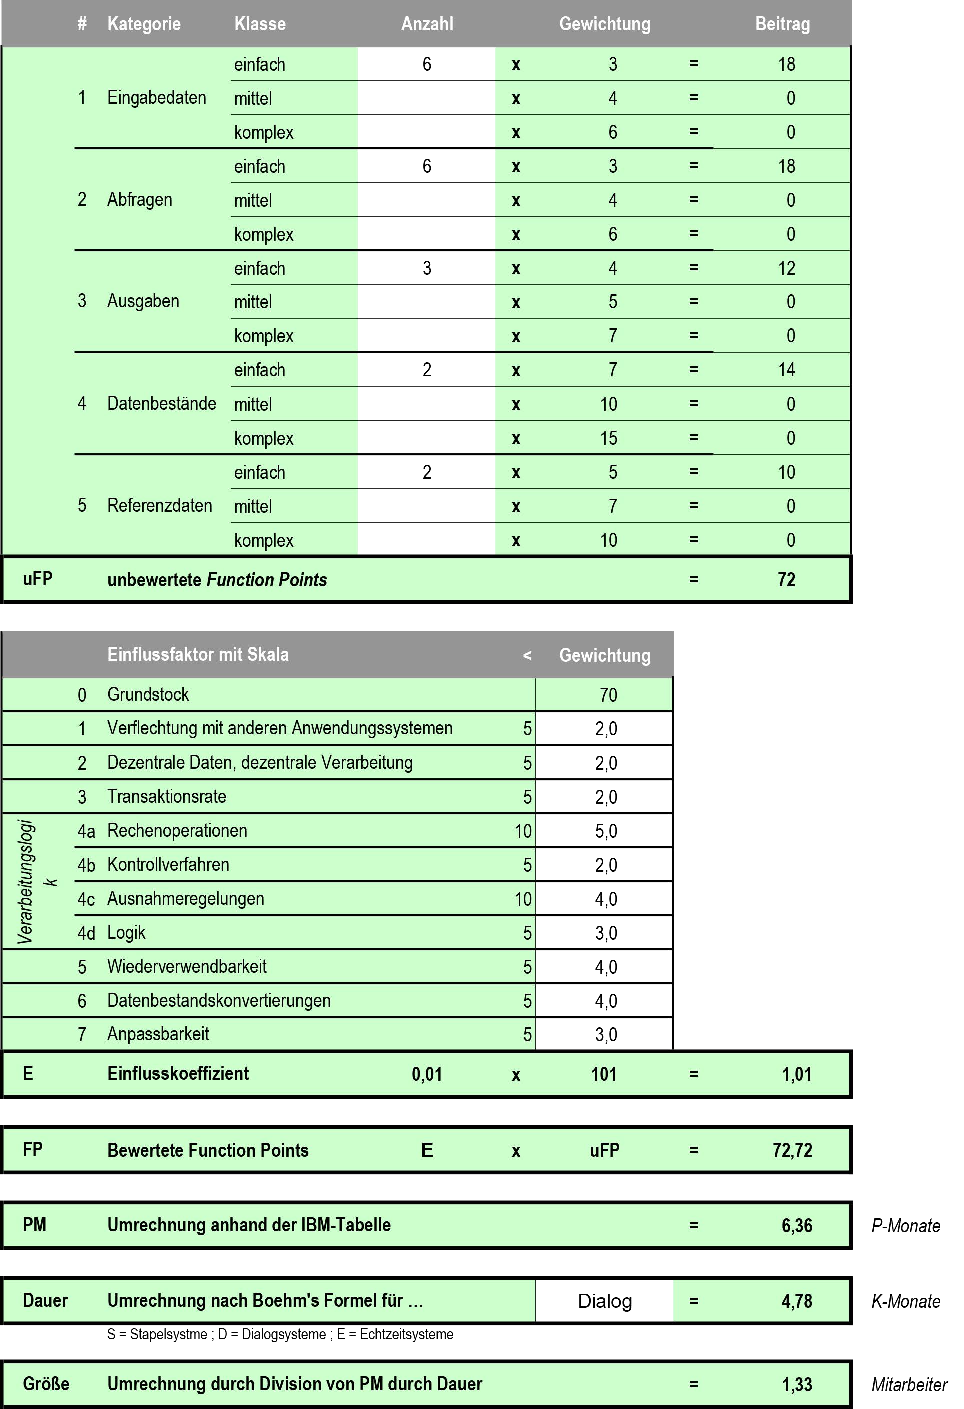
\includegraphics[width=0.9\textwidth]{./files/Aufwand}
	\label{fig:Aufwand}
	\end{figure}

  \end{appendix}

			  
\end{document}